\documentclass[a4paper]{article}

%\usepackage{fullpage}
\usepackage[14pt]{extsizes}			% размер шрифта
\usepackage[T2A]{fontenc}			% кодировка
\usepackage[utf8]{inputenc}			% кодировка исходного текста
\usepackage[english,russian]{babel}	% локализация и переносы
\usepackage{mathtools}				% математический пакет (включает ams)
\usepackage{amssymb}				% для \leqslant
\usepackage[thinc]{esdiff}			% производные
\usepackage{graphicx}				% изображения
\usepackage{wrapfig}				% Обтекание рисунков и таблиц текстом
\usepackage{listings}				% програмный код
\lstset{
	numbers=left               
}
\usepackage{setspace}
\onehalfspacing						% полуторный интервал

\usepackage{tocloft}				% точки в содержании для \section
\renewcommand{\cftsecleader}{\cftdotfill{\cftdotsep}}
\usepackage{siunitx}				% единицы СИ 
									%Number only: \num{1e-10}
									%Number with units: \SI{1e-10}{\meter\per\second}
\author{Бартая Нодари ФМ-101}
\title{ОТЧЁТ\\ Отчёт о НИР}
\date{\today}

\begin{document}
	\section{Основные уравнения}
	%Potter p.272
	Уравнения идеальной гидродинамики в дифференциальной форме относительно неподвижной системы отсчёта:
	\begin{gather}
		\diffp{\rho}{t} + \nabla ( \rho \mathbf{v} ) = 0 ,	\\[10pt]
		\diffp{\rho \mathbf{v}}{t} + (\nabla \rho \mathbf{v}) \mathbf{v} = -\nabla p ,	\\[10pt]
		\diffp{}{t}\left(\rho \varepsilon + \frac{1}{2} \rho v^2 \right) + 
						\nabla \left\{ \left( \frac{1}{2} \rho v^2 + \rho \varepsilon + p \right)\mathbf{v}\right\} = 0 ,
	\end{gather}
	где $\varepsilon$ -- удельная внутренняя энергия. Для иделального газа она выражается как:
	\begin{equation}
		\varepsilon = \dfrac{kT}{m(\gamma-1)} = \dfrac{p}{\rho (\gamma - 1)} ,
	\end{equation}
	где $\gamma$ -- показатель адиабаты (отношение теплоемкостей), $m$ -- масса молекулы (либо атома), $k$ -- постоянная Больцмана, $T$ - температура. 

	\section{Задача о гидродинамическом разрыве}
	%Potter p.319
	Уравнения гидродинамики можно записать в консервативной форме следующим образом:
	\begin{equation}
		\diffp{\mathbf{u}}{t} + \diffp{\mathbf{F}}{x} = 0 ,
	\end{equation}
	где векторы физических величин и потоков равны, соответственно:
	\begin{equation}
	\mathbf{u}	=	\begin{vmatrix}
						\rho								\\
						\rho v								\\
						\frac{1}{2}\rho v^2 + \rho \varepsilon		
					\end{vmatrix} , \qquad	
	\mathbf{F}	=	\begin{vmatrix}
						\rho v								\\
						\rho v^2 + p								\\
						\left(\rho \varepsilon + \frac{1}{2}\rho v^2 + p\right)v	
	\end{vmatrix}	.		
	\end{equation}
	
	\section{Двухшаговый метод Лакса-Вендроффа}
	Рассматриваемый в этом разделе метод является явным, консервативным методом второго порядка точности как по пространству, так и по времени. Непрерывные производные аппроксимируются конечными разностями, далее вычисление проходит в два этапа - предиктор, корректор. 
	
	Первый этап также называют вспомогательным шагом, он производится на каждом шаге по времени и позволяет получить значения величин и их потоков в промежуточные моменты времени, тем самым центрируя по времени интеграл и позволяя получить точность второго порядка. 
	
	\textit{Вспомогательный шаг:}
	\begin{equation}
		\mathbf{u}_{j+1/2}^{n+1/2} = \frac{1}{2} \left(\mathbf{u}_{j}^{n} + \mathbf{u}_{j+1}^{n}\right)
						- \frac{\Delta t}{2 \Delta x}
						\left(\mathbf{F}_{j+1}^{n} - \mathbf{F}_{j}^{n}\right) .
	\end{equation}
	Далее, полученные значения используются для нахождения потоков в промежуточных временных и пространственных точках:
	\begin{equation}
		\mathbf{F}_{j+1/2}^{n+1/2} = \mathbf{F} \left( \mathbf{u}_{j+1/2}^{n+1/2} \right).
	\end{equation}
	На втором этапе, используя промежуточные величины, вычисляется новый временной слой, центрированный по пространству и времени (см. рис \ref{LW_picture}).
	
	\textit{Основной шаг:}
	\begin{equation}
		\mathbf{u}_{j}^{n+1} = \mathbf{u}_{j}^{n} - \frac{\Delta t}{\Delta x} \left(
		\mathbf{F}_{j+1/2}^{n+1/2} - \mathbf{F}_{j-1/2}^{n+1/2}				 \right) .
	\end{equation}
	Условием устойчивости метода является так называемое число Куранта $C \leqslant 1$, что равносильно условию Куранта -- Фридрихса -- Леви, применимого ко всем уравнением гиперболического типа: %(см. стр. 84, 92)
	\begin{equation}
		\Delta t \leqslant \dfrac{\Delta x}{|v|} \:,
	\end{equation}
	где $v$ - наибольшая скорость распространения возмущений на сетке.
	\begin{figure}
		\centering
		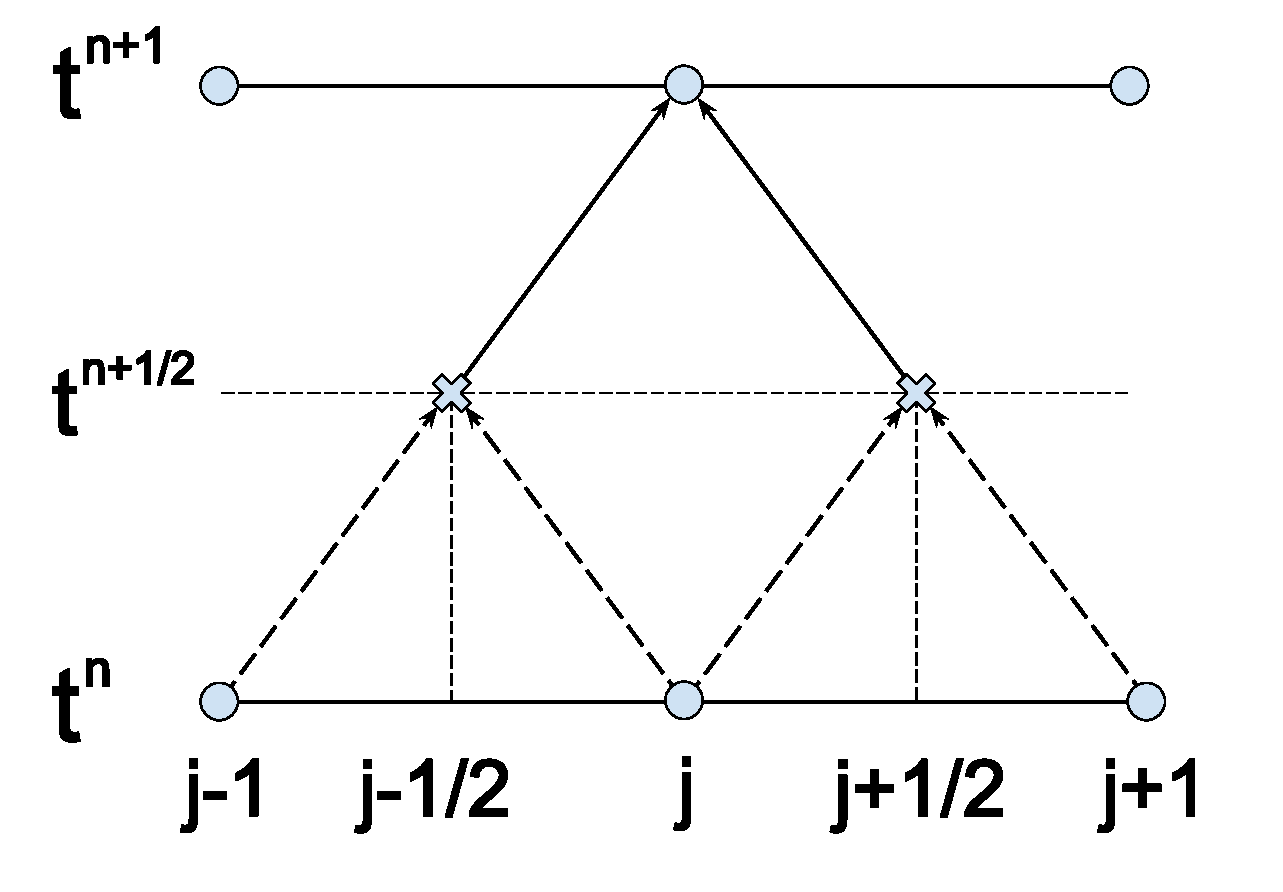
\includegraphics[width=0.8\textwidth]{Lax-Wendroff.pdf}
		\caption{Консервативный двухшаговый метод Лакса-Вендроффа на пространственно - временной сетке.}
		\label{graph_t}
	\end{figure}
\end{document}